\chapter{The Monte-Carlo Method}
Some problems are just too complex to be solved exactly.  Often, these problem can be solved approximately via simulation.
\begin{enumerate}
\item The computation of the volume of a three-dimensional object can be reduced to the computation of a
      \href{https://en.wikipedia.org/wiki/Multiple_integral}{multiple integral}.
      However, if the object has a complicated surface, then computing the associated multiple integral exactly
      might be very difficult.
      In this case, the \href{https://en.wikipedia.org/wiki/Monte_Carlo_integration}{Monte-Carlo} method is
      often able to compute a rough approximation of the volume.  Although the precision attained using the Monte-Carlo
      method is limited, the method is often very easy to implement.
\item Complex systems that are influenced by random events are inherently difficult to predict.  In many cases,
      their behaviour can only be understood via random simulations.  For example, if a new underground transportation system
      is planned, the capacity of the system is estimated via simulation.
\item In games of chance it is sometimes either impossible or at least very difficult to compute the
      probabilities exactly.  However, Monte-Carlo simulations can be used to compute reasonable estimates of these probabilities.
\end{enumerate}
This list can easily be extended.  In this chapter, we investigate three applications of the Monte-Carlo method.
\begin{enumerate}
\item As an introductory example we show how the Monte-Carlo method can be used to compute the area of a
      circle.  This way, the number \href{https://en.wikipedia.org/wiki/Pi}{$\pi$} can be approximated via a simulation.
\item The \href{https://en.wikipedia.org/wiki/Monty_Hall_problem}{Monty Hall problem} is a brain teaser that
      has puzzled a lot of people.  In my personal experience I have found it easiest to convince people via
      a simulation.
\item The final example shows how cards can be randomly shuffled.  This can be used to compute the probability
      that a given \href{https://en.wikipedia.org/wiki/Poker}{Poker} hand wins against a random hand.
\end{enumerate}

\section{How to Compute $\pi$ via Simulation}
The \href{https://en.wikipedia.org/wiki/Unit_circle}{unit circle} $U$ is defined as the set 
\\[0.2cm]
\hspace*{1.3cm}
$U := \bigl\{ \pair(x,y) \in \mathbb{R}^2 \mid x^2 + y^2 \leq 1 \bigr\}$.
\\[0.2cm]
The set $U$ contains those points $\pair(x,y)$ that have distance of $1$ or less from the origin
$\pair(0,0)$.  The unit circle is a subset of the square $Q$ that is defined as 
\\[0.2cm]
\hspace*{1.3cm}
$Q := \bigl\{ \pair(x,y) \in \mathbb{R}^2 \mid -1 \leq x \leq +1 \wedge -1 \leq y \leq +1 \bigr\}$.
\\[0.2cm]
A simple algorithm to compute $\pi$ works as follows:  We randomly throw $n$ grains of sand into the square $Q$.
Then we count the number of grains that end up in the unit circle $U$.  Call this number $k$.
It is reasonable to assume that approximately $k$ is to $n$ as the area of $U$ is to the area of $Q$.  As the area of $Q$ is
$2 \cdot 2$ and the area of $U$ equals $\pi \cdot 1^2$, we should have
\\[0.2cm]
\hspace*{1.3cm}
$\ds\frac{k}{n} \approx \frac{\pi}{4}$.
\\[0.2cm]
Multiplying by $4$ we get
\\[0.2cm]
\hspace*{1.3cm}
$\ds \pi \approx 4 \cdot \frac{k}{n}$.
\\[0.2cm]
Now instead of using grains of sand we can run a simulation.  Figure \ref{fig:Monte-Carlo-Pi.ipynb} on page
\pageref{fig:Monte-Carlo-Pi.ipynb} shows the resulting program.


\begin{figure}[!ht]
\centering
\begin{minted}[ frame         = lines, 
                framesep      = 0.3cm,
                bgcolor       = sepia,
                numbers       = left,
                numbersep     = -0.2cm,
                xleftmargin   = 0.8cm,
                xrightmargin  = 0.8cm,
              ]{python3}
    def approximate_pi(n):
        k = 0
        for _ in range(n):
            x = 2 * rnd.random() - 1
            y = 2 * rnd.random() - 1
            r = x * x + y * y
            if r <= 1:
                k += 1
        return 4 * k / n
\end{minted}
\vspace*{-0.3cm}
\caption{Computing $\pi$ using the Monte-Carlo method.}
\label{fig:Monte-Carlo-Pi.ipynb}
\end{figure}

\begin{enumerate}
\item The parameter $n$ specifies the number of grains of sand that are thrown into the square $Q$.
\item In order to throw a grain of sand randomly into $Q$ we first compute random numbers using the function
      $\mytt{random}()$.  These random numbers are distributed uniformly in the interval  $[0,1]$.   The
      transformation  
      \\[0.2cm]
      \hspace*{1.3cm}
      $t \mapsto 2 \cdot t - 1$
      \\[0.2cm]
      maps the interval $[0,1]$ into the interval $[-1, 1]$.  Hence, the coordinates $\mytt{x}$ und
      $\mytt{y}$ that are computed in the lines 5 and 6 represent a random point $\pair(\mytt{x}, \mytt{y})$ 
      in the square $Q$.
\item Line  7 computes the square of the distance between $\pair(x,y)$ and $\pair(0,0)$.  If this distance is
      less or equal than 1, then the point $\pair(x,y)$ is inside the unit circle $U$.  In this case, the counter $k$ is incremented.
\end{enumerate}

\begin{table}[htbp]
  \label{tab:pi}
  \centering
  \begin{tabular}[t]{|r|r|r|}
  \hline
  n & approximation of $\pi$ & absolute error \\
  \hline
  \hline
               $10$ & 2.40000 & -0.741593 \\
\hline
              $100$ & 3.28000 & +0.138407 \\
\hline
           $1\,000$ & 3.21600 & +0.074407 \\
\hline
          $10\,000$ & 3.13080 & -0.010793 \\
\hline
         $100\,000$ & 3.13832 & -0.003273 \\
\hline
      $1\,000\,000$ & 3.13933 & -0.002261 \\
\hline
     $10\,000\,000$ & 3.14095 & -0.000645 \\
\hline
    $100\,000\,000$ & 3.14155 & -0.000042 \\
\hline
 $1\,000\,000\,000$ & 3.14160 & +0.000011 \\
\hline
  \end{tabular}
  \caption{Results for the approximate computation of $\pi$ using a Monte-Carlo simulation.}
\end{table}

If we run this program, we get the results shown in table \ref{tab:pi} on page \pageref{tab:pi}.
In order to compute $\pi$ with a precision of $10^{-3}$ we need about $10\,000\,000$ trials.  Given the
computational power of modern computers this number can be achieved within seconds.  However,  if we need more
precision, things get harder:  In order to achieve an error less than  $10^{-4}$ we already need
$1\,000\,000\,000$ trials.  Every time that we want to increase the precision by a factor of ten, we need to
increase the number of trial by a hundred times!


\begin{center}
\colorbox{red}{\framebox{\colorbox{orange}{
  \begin{minipage}[t]{12cm}
  Monte-Carlo simulations are efficient as long as only rough estimates are needed.  However, if we need high
  precision results, the Monte-Carlo method gets inefficient.
  \end{minipage}
  }}}
\end{center}

% \section[Theory]{Theoretischer Hintergrund$^*$}
% Wir diskutieren nun den theoretischen Hintergrund der Monte-Carlo-Methode.  Da im zweiten Semester noch
% keine detaillierteren Kenntnisse aus der Wahrscheinlichkeits\-rechnung vorhanden sind, beschr\"anken wir
% uns darauf, die wesentlichen Ergebnisse anzugeben.  Eine Begr\"undung dieser Ergebnisse erfolgt dann
% in der Statistik-Vorlesung im vierten Semester. 

% Bei der Monte-Carlo-Methode wird ein Zufalls-Experiment, im gerade diskutierten Beispiel war es das Werfen
% eines Sandkorns, sehr oft wiederholt.  F\"ur den Ausgang dieses Zufalls-Experiments gibt es dabei zwei
% M\"oglichkeiten:  Es ist ent\-weder erfolgreich (im obigen Beispiel landet das Sandkorn im Kreis) oder nicht
% erfolgreich.  Ein solches Experiment bezeichnen wir als \emph{Bernoulli-Experiment}.
%  Hat die Wahrscheinlichkeit, dass das Experiment erfolgreich ist, den Wert $p$ und wird das
% Experiment $n$ mal ausgef\"uhrt, so ist die Wahrscheinlichkeit, dass genau $k$ dieser Versuche erfolgreich sind,
% durch die Formel
% \[ P(k) = \frac{n!}{k! \cdot (n-k)!} \cdot p^k \cdot (1-p)^{n-k} \]
% gegeben, die auch als \emph{Binomial-Verteilung} bekannt ist.  F\"ur gro{\ss}e Werte von $n$ ist die obige Formel
% sehr unhandlich, kann aber gut durch die \emph{Gau{\ss}-Verteilung} approximiert werden, es gilt
% \\[0.2cm]
% \hspace*{0.8cm}
% $\ds\frac{n!}{k! \cdot (n-k)!} \cdot p^k \cdot (1-p)^{n-k} \approx  
%    \frac{1}{\sqrt{2\cdot \pi \cdot n \cdot p \cdot (1-p)\;}} \cdot 
%    \exp\left(-\frac{(k - n \cdot p)^2}{2 \cdot n \cdot p \cdot (1 - p)}\right)
% $
% \\[0.2cm]
% Wird das Experiment $n$ mal durchgef\"uhrt, so erwarten wir im Durchschnitt nat\"urlich, dass $n \cdot p$ der
% Versuche erfolgreich sein werden.  Darauf basiert unsere Sch\"atzung f\"ur den Wert von $p$, denn wir approximieren
% $p$ durch die Formel
% \[ p \approx \frac{k}{n}, \]
% wobei $k$ die Anzahl der erfolgreichen Experimente bezeichnet.  Nun werden in der Regel nicht genau $n \cdot p$
% Versuche erfolgreich sein: Zufallsbedingt werden etwas mehr oder etwas weniger Versuche
% erfolgreich sein.  Das f\"uhrt dazu, dass unsere Sch\"atzung von $p$ eine Ungenauigkeit aufweist, deren ungef\"ahre
% Gr\"o{\ss}e wir irgendwie absch\"atzen m\"ussen um unsere Ergebnisse beurteilen zu k\"onnen.

% Um eine Idee davon zu bekommen, wie sehr die Anzahl der erfolgreichen Versuche von dem Wert $\frac{k}{n}$
% abweicht,  f\"uhren wir den Begriff der \emph{Streuung} $\sigma$ ein, die f\"ur eine binomialverteilte Zufallsgr\"o{\ss}e
% durch die Formel
% \[ \sigma = \sqrt{n \cdot p \cdot (1 - p)} \]
% gegeben ist.  Die Streuung gibt ein Ma{\ss} daf\"ur, wie stark der gemessene Wert von $k$ von dem im Mittel
% erwarteten Wert $p \cdot n$ abweicht.  Es kann gezeigt werden, dass die Wahrscheinlichkeit, dass $k$ au{\ss}erhalb
% des Intervalls
% \[ [ p \cdot n - 3 \cdot \sigma,\, p \cdot n + 3 \cdot \sigma ] \]
% liegt, also um mehr als das Dreifache von dem erwarteten Wert abweicht, kleiner als $0.27 \%$ ist.  F\"ur
%  die Genauigkeit unserer Sch\"atzung $p \approx \frac{k}{n}$ hei{\ss}t das, dass dieser Sch\"atzwert mit hoher
%  Wahrscheinlichkeit ($99.73\%$) in dem Intervall
% \[  \left[ \frac{p \cdot n - 3 \cdot \sigma}{n},\, \frac{p \cdot n + 3 \cdot \sigma}{n} \right] 
%   = \left[ p - 3 \cdot \frac{\sigma}{n},\, p + 3 \cdot \frac{\sigma}{n} \right]
% \] 
% liegt.  Die Genauigkeit $\varepsilon(n)$ ist durch die halbe L\"ange dieses Intervalls gegeben und hat daher den
% Wert 
% \[ \varepsilon(n) = 3 \cdot \frac{\sigma}{n} = 3 \cdot \sqrt{\frac{p \cdot (1 - p)}{n}}. \]
% Wir erkennen hier, dass zur Erh\"ohung der Genauigkeit um den Faktor 10 die Zahl der Versuche um den Faktor 100
% vergr\"o{\ss}ert werden muss.

% Wenden wir die obige Formel auf die im letzten Abschnitt durchgef\"uhrte Berechnung der Zahl $\pi$ an, so erhalten
% wir wegen $p = \frac{\pi}{4}$ die in Abbildung \ref{tab:Precision.java} gezeigten Ergebnisse.

% \begin{table}[htbp]
%   \centering
%   \begin{tabular}[t]{|r|r|}
% \hline
% Anzahl Versuche $n$ & Genauigkeit $\varepsilon(n)$ \\
% \hline
% \hline
%                 $10$ & 0.389478 \\
% \hline
%                $100$ & 0.123164 \\
% \hline
%             $1\,000$ & 0.0389478 \\
% \hline
%            $10\,000$ & 0.0123164 \\
% \hline
%           $100\,000$ & 0.00389478 \\
% \hline
%        $1\,000\,000$ & 0.00123164 \\
% \hline
%       $10\,000\,000$ & 0.000389478 \\
% \hline
%      $100\,000\,000$ & 0.000123164 \\
% \hline
%   $1\,000\,000\,000$ & 3.89478e-05 \\
% \hline
%  $10\,000\,000\,000$ & 1.23164e-05 \\
% \hline
% $100\,000\,000\,000$ & 3.89478e-06 \\
% \hline

%   \end{tabular}
%   \caption{Genauigkeit der Bestimmung von $\pi$ bei einer Sicherheit von $99,73\%$.}
%   \label{tab:Precision.java}
% \end{table}

% \vspace*{0.3cm}

% \exercise
% Wie viele Versuche sind notwendig um $\pi$ mit der Monte-Carlo-Methode auf 6
% Stellen hinter dem Komma zu berechnen, wenn das Ergebnis mit einer Wahr\-scheinlichkeit von $99,73\%$
% korrekt sein soll?
% \vspace*{0.1cm}

% \noindent
% \textbf{Hinweis}: 
% Um eine Genauigkeit von 6 Stellen hinter dem Komma zu erreichen, sollte der Fehler durch $10^{-7}$
% abgesch\"atzt werden.  \eox
% \pagebreak

% \solution
% Nach dem Hinweis soll 
% \\[0.2cm]
% \hspace*{1.3cm}
% $\varepsilon(n) = 10^{-7}$
% \\[0.2cm]
% gelten. Setzen wir hier die Formel f\"ur $\varepsilon(n)$ ein, so erhalten wir
% \\[0.2cm]
% \hspace*{1.3cm}
% $  
% \begin{array}[t]{llcl}
%                 & \ds 3 \cdot \sqrt{\frac{p \cdot (1 - p)}{n}} & = & 10^{-7}   \\[0.3cm]
% \Leftrightarrow & \ds 9 \cdot        \frac{p \cdot (1 - p)}{n} & = & 10^{-14}      \\[0.3cm]
% \Leftrightarrow & \ds 9 \cdot    p \cdot (1 - p) \cdot 10^{14} & = & n 
% \end{array}
% $
% \\[0.2cm] 
% Um an dieser Stelle weitermachen zu k\"onnen, ben\"otigen wir den Wert der Wahr\-scheinlichkeit $p$.  Der korrekte
% Wert von $p$ ist f\"ur unser Experiment durch $\frac{\pi}{4}$ gegeben.  Da wir $\pi$ ja erst berechnen wollen,
% nehmen wir als N\"aherung von $\pi$ den Wert $3$, so dass $p$ den Wert $\frac{3}{4}$ hat.  Damit
% ergibt sich f\"ur $n$ der Wert
% \\[0.2cm]
% \hspace*{1.3cm}
% $n = 168.75 \cdot 10^{12}$.
% \\[0.2cm]
% Das sind also mehr als fast 169 Billionen Versuche. \qed


% \exercise
% Berechnen Sie mit Hilfe der Monte-Carlo-Methode eine N\"aherung f\"ur den Ausdruck $\mathrm{ln}(2)$.
% Ihre N\"aherung soll mit einer Wahrscheinlichkeit von $99.73\%$ eine Genauigkeit von 
% $\varepsilon = 10^{-3}$ haben. \eox


\section{The Monty Hall Problem}
The \href{http://en.wikipedia.org/wiki/Monty_Hall_problem}{Monty Hall problem} is a famous probability
puzzle that is based on the TV show 
\href{http://en.wikipedia.org/wiki/Let%27s_Make_a_Deal}{Let's Make a Deal}, which was aired in the
US from the sixties through the seventies.  The host of this show was 
\href{http://en.wikipedia.org/wiki/Monty_Hall}{Monty Hall}. In his show, a player had to choose one
of three doors.  Monty Hall had placed goats behind two of the doors but there was a shiny new car
behind the third door.  Of course, the player did not know the location of the door with the car.  
Once the player had told Monty Hall the door she had chosen, Monty Hall would open one of the other
two doors.  However, Monty Hall would never open the door with the car behind it.  Therefore, if the
player had chosen the door with the car, Monty Hall would have randomly chosen a door leading to a
goat.  If, instead, the player had chosen a door leading to a goat, Monty Hall would have opened the
door showing the other goat.  In either case, after opening the door  Monty Hall would ask the
player whether she wanted to stick with her first choice or whether, instead, she wanted to pick the
remaining closed door.  Figure \ref{fig:monty-hall} on page \pageref{fig:monty-hall} shows what happens if we
open the wrong door.

\begin{figure}[!t]
  \centering
  \framebox{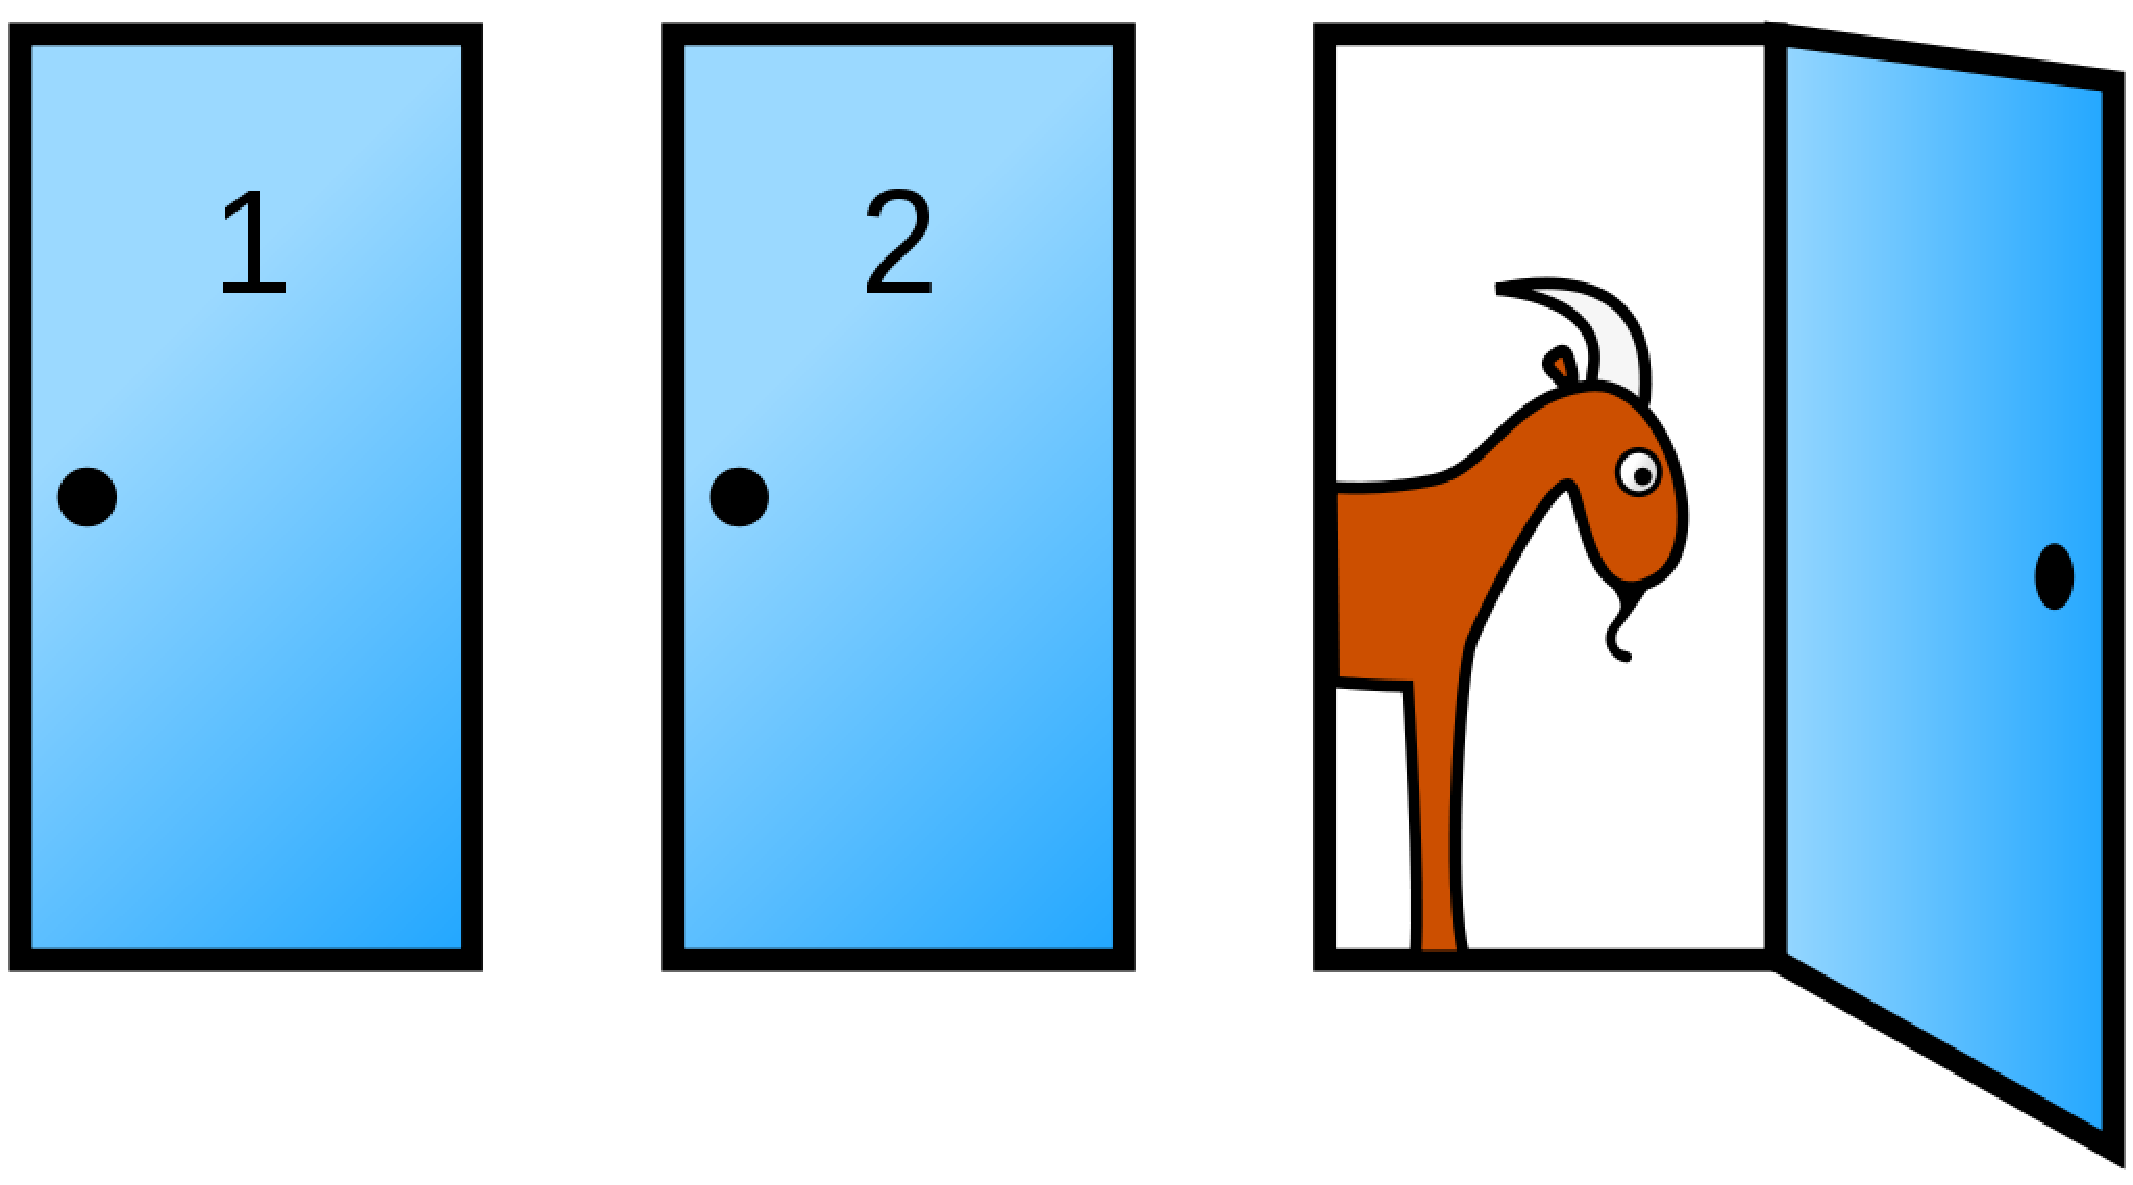
\epsfig{file=Abbildungen/monty-hall,scale=0.3}} 
  \caption{Opening the wrong door.}
  \label{fig:monty-hall}
\end{figure}


In order to better understand the problem you can try the animation at:
\\[0.2cm]
\hspace*{1.3cm}
\href{https://www.mathwarehouse.com/monty-hall-simulation-online/}{\texttt{https://www.mathwarehouse.com/monty-hall-simulation-online/}}
\\[0.2cm]
The question now is whether it is a good strategy to stick with the door chosen first or whether it
is a better idea to switch doors.  Mathematically, the reasoning is quite simple: As there are three doors
initially and the probability that the car is behind any of them is the same, the probability that the
door chosen first leads to the car is $\frac{1}{3}$.  Therefore, the probability that the car is behind
the other unopened door has to be $\frac{2}{3}$, as the two probabilities have to add up to $1$.  Hence the
best strategy is to switch the door.

Although the reasoning given above is straightforward, many people don't believe it, as is shown
by this \href{https://priceonomics.com/the-time-everyone-corrected-the-worlds-smartest/}{article}.  In order to
convince them, the best thing is to run a Monte Carlo simulation.  Figure \ref{fig:Monty-Hall-Problem.ipynb}
on page 
\pageref{fig:Monty-Hall-Problem.ipynb} shows a function that simulates \mytt{n} games and compares the
different strategies.  
\begin{enumerate}
\item The first strategy is the strategy that does not switch doors.
      This strategy is called the \blue{persistent strategy}.
\item The second strategy will always switch to the other door.
      This strategy is called the \blue{wavering strategy}.
\end{enumerate}

\begin{figure}[!ht]
\centering
\begin{minted}[ frame         = lines, 
                framesep      = 0.3cm, 
                firstnumber   = 1,
                bgcolor = sepia,
                numbers       = left,
                numbersep     = -0.2cm,
                xleftmargin   = 0.8cm,
                xrightmargin  = 0.8cm,
              ]{python3}
    def calculate_chances(n):
        success_persistent = 0
        success_wavering   = 0
        for _ in range(n):
            car    = rnd.randint(1, 3)
            choice = rnd.randint(1, 3) 
            opened = rnd.choice(list({1, 2, 3} - {choice, car}))
            last   = arb({ 1, 2, 3 } - { choice, opened })
            if car == choice:
                success_persistent += 1
            if car == last:
                success_wavering  += 1
        print(f'The persistent strategy wins {success_persistent} cars.')
        print(f'The wavering   strategy wins {success_wavering  } cars.')
\end{minted}
\vspace*{-0.3cm}
\caption{A program to solve the Monty Hall problem.}
\label{fig:Monty-Hall-Problem.ipynb}
\end{figure}
\FloatBarrier

    
We discuss the implementation of the function \mytt{calculate\_chances} line by line.
\begin{enumerate}
\item In order to compare the two strategies, the idea is to play the game offered by Monty Hall
      \mytt{n} times.  Then we need to count how many cars are won by the persistent strategy and how
      many cars are won by the wavering strategy.
\item The variable \mytt{success\_persistent} counts the number of cars won by the persistent strategy.
\item The variable \mytt{success\_wavering}  counts the number of cars won by the wavering  strategy.
\item The \mytt{for} loop extending from line 4 to line 12 runs \mytt{n} simulations of the
       game.
       \begin{enumerate}
       \item First, in line 5 the car is placed randomly behind one of the three doors.
       \item Second, in line 6 the player picks a door.
       \item In line 7, Monty Hall opens a door that does not have a car behind it and that
             is different from the door chosen by the player.
       \item When the player uses the wavering strategy, she will then pick the remaining door in line 8.
       \end{enumerate}
\item Next, we check which of the two strategies actually wins the car.
      \begin{enumerate}
      \item If the car was placed behind the door originally chosen by the player, the persistent
            strategy wins the car.  Therefore, we increment the variable \mytt{success\_persistent} in
            this case.
      \item If, instead, the car was placed behind the door that was neither chosen nor opened, then
            the wavering strategy wins the car.  Hence, the variable \mytt{success\_wavering} has to be incremented.
      \end{enumerate}
\item The function concludes by printing the results.  Running the function for \mytt{n} equal to
      $1000\,000$ has yielded the following result:
      \\[0.2cm]
      \hspace*{1.3cm}
      \mytt{The persistent strategy wins 333525 cars.} \\ 
      \hspace*{1.3cm}
      \mytt{The wavering \ \ strategy wins 666475 cars.}
      \\[0.2cm]
      This shows that, on average, the payoff from the wavering strategy is about twice as high as the
      payoff from the persistent strategy.  This is just what we expect since $\frac{2}{3} = 2 \cdot \frac{1}{3}$.
\end{enumerate}

\section[Permutations]{Generation of Random Permutations}
In this section we present an algorithm that can randomly permute a given list.
Such a procedure can be likened to the shuffling of cards. The process is actually used for this purpose: When
calculating the probability of winning in card games such as poker, the cards are shuffled using the algorithm
presented here. 

In order to permute a list $L = [x_1,x_2, \cdots, x_n]$ of length $n$ we distinguish two cases:
\begin{enumerate}
\item The list  $L$ has length 1 and hence contains a single element, i.e.~we have $L = [x]$.
      In this case,  $\mytt{permute}(L)$ returns the list unchanged:
      \\[0.2cm]
      \hspace*{1.3cm}
      $\#L = 1 \rightarrow \mytt{permute}(L) = L$.
\item The length of  $L$ is bigger than  $1$.  In this case, we randomly select an element to be the last in
      the permutation to be created.  We remove this element from the list and then permute the remaining list.  
      We append the initially selected element to the resulting permutation.
      Given two natural numbers $a$ and $b$ such that $a < b$ the \textsl{Python} function
      \\[0.2cm]
      \hspace*{1.3cm}
      $\mytt{rnd.randint}(a,b)$
      \\[0.2cm]
      returns a random element from the set $\{a,\cdots,b\}$.  Using this function we define:
      \\[0.2cm]
      \hspace*{0.8cm}
      $\#L = n \wedge n > 1 \wedge k :=\mytt{rnd.randint}(0,n-1) $
      \\[0.2cm]
      \hspace*{2.3cm}
      $\rightarrow\quad  
         \mytt{permute}(L) = \mytt{permute}\bigl(L\mytt{[:}k\mytt{]} + L\mytt{[}k+1\mytt{:]}\bigr) + \mytt{[}L\mytt{[}k\mytt{]]}
      $.
\end{enumerate}

\begin{figure}[!ht]
\centering
\begin{minted}[ frame         = lines, 
                framesep      = 0.3cm,
                bgcolor = sepia,
                numbers       = left,
                numbersep     = -0.2cm,
                xleftmargin   = 0.8cm,
                xrightmargin  = 0.8cm,
              ]{python3}
    def permute(L):
        if len(L) == 1:
            return L
        k = rnd.randint(0, len(L)-1)
        return permute(L[:k] + L[k+1:]) + [L[k]]
\end{minted}
\vspace*{-0.3cm}
\caption{Computation of random permutations of a list.}
\label{fig:Permutation.ipynb}
\end{figure}

Figure \ref{fig:Permutation.ipynb} shows the implementation of this idea in Python. The method \texttt{permute} shown
there creates a random permutation of the list $L$, which is passed as argument. The implementation directly
implements the equations described above. 

It can be shown that the algorithm presented above actually generates all permutations of a given list with the
same probability. A proof of this claim can be found, for example, in 
Cormen et.~al.~\cite{cormen:01}.



%%% LOCAL Variables: 
%%% mode: latex
%%% TeX-master: "algorithms"
%%% End: 
